
%\section{Architecture}
\begin{figure}[htbp]
\centering % 使图片居中对齐
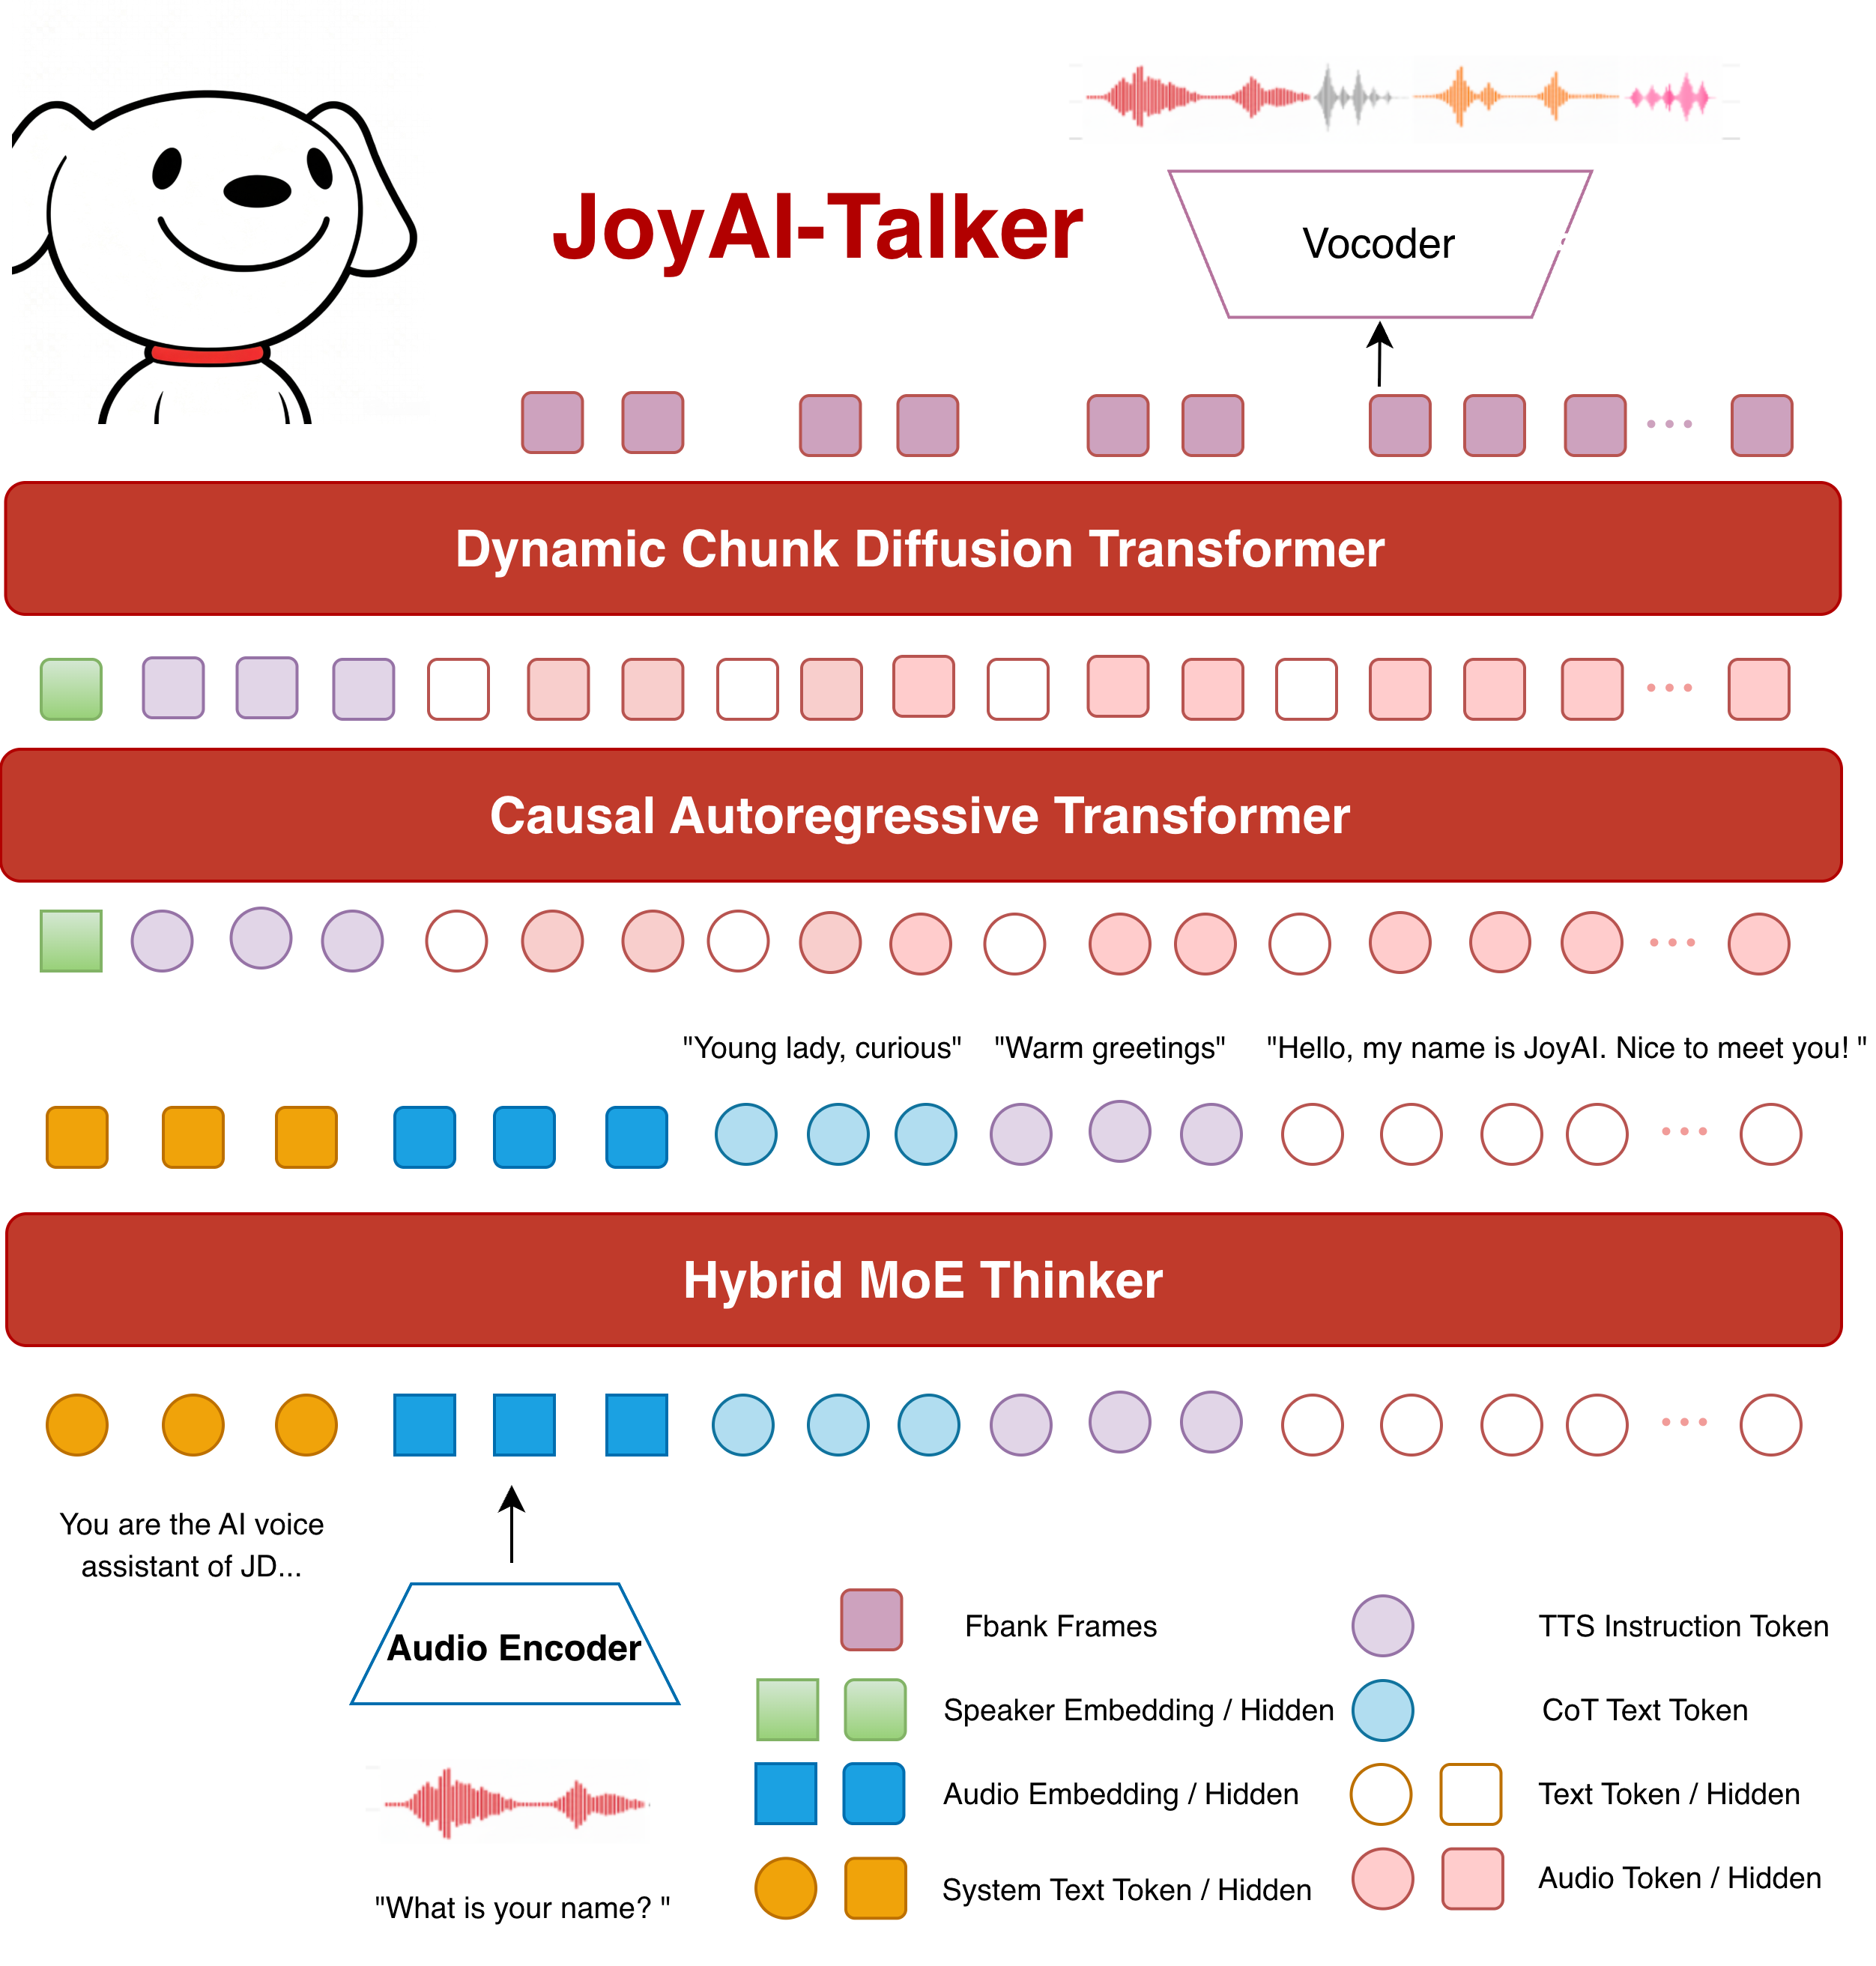
\includegraphics[width=0.85\textwidth]{pic/talker_stream_v2.png}
\caption{An overview of Thinker-Talker pipeline in JoyAI-Talker. It consists of several key components: 
1) Audio Encoder: This module processes the input speech query and extracts continuous audio embeddings. 
2) Hybrid MoE Thinker: Ingesting multimodal inputs, this cognitive core performs reasoning to predict the target text tokens and TTS instruction tokens. 
3) Causal Autoregressive Transformer: This module takes the speaker embeddings, predicted TTS instruction tokens, and target text tokens as input, and predicts the discrete audio tokens. 
4) Dynamic Chunk Diffusion Transformer: Using the hidden representations from the Causal Autoregressive Transformer as input, this component predicts the mel-spectrogram output. 
5) Vocoder: This module is responsible for reconstructing the predicted mel-spectrogram back to continuous waveform audio.} % 图片下方的标题
\label{fig:example} % 标签，用于在正文中引用该图片
\end{figure}
\section{Duplex-Thinker-Talker Architecture}
JoyAI-Talker is designed as a decoupled, state-driven, full-duplex speech dialogue system structured around three core pillars: the \textbf{Duplex Interaction}, the \textbf{Thinker}, and the \textbf{Talker}. Unlike computationally heavy, end-to-end parallel dual-stream architectures, this modular paradigm separates conversational state coordination, cognitive semantic reasoning, and expressive acoustic synthesis. By establishing a clear separation of concerns, the system achieves a balanced trade-off between semantic intelligence, acoustic expressiveness, and engineering deployability.

\paragraph{Architectural Advantages:}
This decoupled modular design offers two major advantages:
\begin{itemize}
    \item \textbf{Modularity and Independent Optimization:} Each component can be trained, fine-tuned, or upgraded independently without retraining the entire end-to-end pipeline. This plug-and-play capability greatly simplifies engineering maintenance and reduces development costs.
    
    \item \textbf{Preservation of Cognitive Capabilities:} In tightly coupled speech dialogue systems, real-time interactive responsiveness often conflicts with deep semantic intelligence. To enable low-latency full-duplex interaction, models must constantly process fine-grained temporal steps, whether through real-time frame prediction over short temporal chunks~\cite{thinkingmachines2026interactionmodels} or continuous dual-stream audio token ingestion as in Moshi-like architectures~\cite{defossez2024moshi}. Integrating these high-frequency, low-level streaming classification tasks directly into the primary language backbone fragments its contextual attention and dilutes its parameter capacity, leading to severe cognitive degradation and a drop in overall reasoning performance. By offloading these rapid, short-chunk state-tracking and interactive routing tasks to the outer Duplex Interaction Layer, our design shields the Thinker's semantic core, allowing it to focus exclusively on coherent, long-context reasoning and empathetic alignment.
\end{itemize}

\paragraph{Limitations and Mitigations:}
Nonetheless, the decoupled paradigm introduces certain engineering and architectural trade-offs:
\begin{itemize}
    \item \textbf{Slightly Higher Latency Overhead:} Sequential routing across modular boundaries (even when optimized via chunk-based streaming) naturally introduces a minor latency penalty, resulting in a slightly higher turn-taking latency than unified, single-pass parallel models.
    
    \item \textbf{Information Bottleneck at the Interface:} The symbolic interface between the Thinker and the Talker prevents the direct propagation of continuous acoustic nuances (such as the user's exact pitch fluctuations or micro-hesitations from the input). We actively mitigate this limitation by generating structured, localized paralinguistic tokens (e.g., \texttt{[Sigh]}, \texttt{[Laughter]}) and emotion-aware speaking instructions. These explicit cues allow the Talker to reconstruct rich emotional prosody in a highly controllable and precise manner.
    
    \item \textbf{Infrastructure Complexity:} Managing asynchronous full-duplex interactions—such as real-time barge-in, voice activation detection (VAD), and stream cancellation—requires a relatively complex, state-driven serving architecture.
\end{itemize}







